\documentclass[a4paper,11pt]{report}
\usepackage[utf8]{inputenc}
\usepackage[english]{babel}
\usepackage[font=small,labelfont=bf, textfont=it]{caption}
%\usepackage[top=1.5cm, bottom=1.5cm, left=2cm, right=2cm]{geometry} % to change padding
\usepackage{geometry}
\usepackage{verbatim}
\usepackage{subcaption} % for multi figure
\usepackage{enumitem} % -- label item
\usepackage{tabularx} % table
\usepackage{color}
\usepackage[usenames, dvipsnames]{xcolor} % color
\usepackage[framemethod=TikZ]{mdframed} % box
\usepackage{listings} % code
%\usepackage{amsmath} % align* maths
\usepackage[bookmarks, hidelinks, linktoc=all]{hyperref} % clickable links
\usepackage{graphicx} % includegraphics
\usepackage{indentfirst} % indentation
\usepackage{titlesec} % spacing between sections
\usepackage{multicol} % multi columns
\usepackage{amssymb}
\usepackage{tikz}
\usetikzlibrary{shapes,arrows}
% \usepackage{tocloft}
%\setlength\cftaftertoctitleskip{50pt} % toc space after title
%\setlength{\cftbeforetoctitleskip}{-3em} % toc space before title

\setlength\parindent{0pt}
\setlength{\parskip}{0.9em} % paragraph vertical space

\renewcommand\thesection{\arabic{section}} % start section from 1
\setcounter{tocdepth}{1} % display subsection in toc
\setcounter{secnumdepth}{3} % number subsubsection

% space before lists
\setlist[itemize]{topsep=0pt}
\setlist[enumerate]{topsep=0pt}

% spacing between figure and caption
% \setlength{\abovecaptionskip}{2pt plus 2pt minus 4pt} % default: 10pt

% Titre
% \title{Distributed Artificial Intelligence \& Intelligent Agents \\ DAIIA - Project}
% \author{Laurentiu CAPATINA \& Quentin LEMAIRE}

\begin{document}

  % first page
  \pagenumbering{Alph}
\begin{titlepage}
  \centering
  \vspace*{\stretch{1}}
  \vfill
    {\bfseries\Large{
	Distributed Artificial Intelligence\\\&\\Intelligent Agents}
    }
  \vfill
  \vfill
    \Huge{\textsc{Smart Museum}}
    \\\vspace{10pt}
    \Large{Project report}
  \vfill
      \Large{\textsc{Laurentiu Capatina} \& \textsc{Quentin Lemaire}}
    \\
  \vspace{0.4cm}
    Group 5
  \vfill
  \vfill
    % \includegraphics[width=0.22\textwidth]{media/kth.jpg}
    KTH Royal Institute of Technology
  \vfill
    \today
  \vspace*{\stretch{1}}
  \thispagestyle{empty}
\end{titlepage}
\pagenumbering{arabic}

\addtocontents{toc}{\protect\thispagestyle{empty}} % remove toc pagination
\tableofcontents{} % toc
\clearpage % leave a page
\setcounter{page}{1} % init counter page

  \section{Introduction}
  % TODO describe aim of the project
  % TODO describe briefly different tasks
  
  This project deals with \textbf{Agent Oriented Software Engineering} (AOSE) in the 
  context of a virtual exhibitions (smart museum). The aim is to model a multi-agent 
  system with specific methods of modelisation: GAIA and Role-base modeling.
  As a consequence of the previous works, this project reuses concepts we learnt 
  during lectures and homeworks: behaviors, messaging, negotiation, mobility, ...
  
  
  %%%%%%
  
  
  \section{GAIA Methodology} % task 1
  % Model your system via GAIA AOSE Methodology
  % Agent Oriented Sofware Engineering (AOSE)
  
  \subsection{Requirements statement}
  % TODO text describing the scenario
  
  In the smart museum scenario, we have different actors: artist managers, curators 
  and profilers.
  
  Firstly, the artist manager is responsible to gather paintings or art creations 
  from a set of different artists he or she is in contact with. The goal of the manager 
  is to sell products with different quality level to profilers.
  
  In order to sell paintings to profilers, the artist manager has to use curators as retailers 
  because they don't know profilers directly. The curators are associated to a museum and there
  is only one for each museum. In our model we have 2 museums and consequently 2 curators. The artist manager 
  provides a product with an announced price to curators who will afterwards
  sell it to profilers. Because there are 2 curators and only one of them can buy 
  the product, curators have to visit the artist manager in order to take part in a Dutch auction. 
  This auction will determine which curator gets the product.
  
  Finally, the profiler receives suggestions of products offered by curators and can choose whether he or 
  she wants to buy the product at the displayed price or not.
  
  % TODO put schemes (the one in instructions ?)
  
  \subsection{Roles model}
  
  Different roles can be modeled in our scenario:
  \begin{itemize}
  \itemsep0pt
   \item Artist Manager role (described in Figure~\ref{figure:role_artist_manager})
   \item Curator role (described in Figure~\ref{figure:role_curator})
   \item Profiler role (described in Figure~\ref{figure:role_profiler})
  \end{itemize}

  % TODO
  \begin{figure}[ht!]
    \begin{mdframed}
      Role Schema: \textsc{Artist Manager} \\ \hrule \vspace{2pt} \hrule \vspace{10pt}
      Description:\\
      Gathers high or low quality products and acts as auctioneer with Curators.
      \\ \hrule \vspace{10pt}
      Protocols and Activities:
      \vspace{-10pt}
      \begin{flushleft}
       \underline{ChooseHighOrLowQualityProduct}, 
       %WaitTwoOrMoreCurators, 
       DutchAuction 
       %WaitMoneyOrProductBack
      \end{flushleft}
      \hrule \vspace{10pt}
      Permissions:\\
      \vspace{-15pt}
      \begin{center}
       generates \textit{painting //new painting to sell}
      \end{center}
      % ask "artist" to product high or low quality product
      % auction product
      \hrule \vspace{10pt}
      Responsabilities:\\
      Liveness:
      \begin{flushleft}
      \small\textsc{Artist Manager} = (\underline{ChooseHighOrLowQualityProduct}, 
      %WaitTwoOrMoreCurators, 
      DutchAuction 
      %WaitMoneyOrProductBack
      )$^\omega$
      \end{flushleft}
      Safety:
      \begin{itemize}
      \itemsep0pt
       \item $money > 0$
       \item $paintings \geq 0$
      \end{itemize}
 % TODO
    \end{mdframed}
  \caption{Artist manager role}
  \label{figure:role_artist_manager}
  \end{figure}
  
  
  \begin{figure}[ht!]
    \begin{mdframed}
      Role Schema: \textsc{Curator} \\ \hrule \vspace{2pt} \hrule \vspace{10pt}
      Description:\\
      This role can be seen as an intermediate for selling paintings between the Profiler
      and the Artist Manager.
      \\ \hrule \vspace{10pt}
      Protocols and Activities:
      \vspace{-10pt}
      \begin{flushleft}
       \underline{DefineStrategy}, DutchAuction,
       \underline{DefineNewPrice},
       ProposeProduct, WaitResponse
      \end{flushleft}
      \hrule \vspace{10pt}
      Permissions:\\
      \vspace{-15pt}
      \begin{center}
       reads \textit{paintingName //name of the painting}\\
	    \textit{offer //offer received for auction}\\
       changes \textit{strategy //strategy for auction}\\
       \textit{paintingPrice //new price for painting}
      \end{center}
      % ask "artist" to product high or low quality product
      % auction product
      \hrule \vspace{10pt}
      Responsabilities:\\
      Liveness:
      \begin{flushleft}
      \small\textsc{Curator} = \underline{DefineStrategy}(DutchAuction, $\mid$\underline{DefineNewPrice},
       ProposeProduct, WaitResponse$\mid$)$^\omega$
      \end{flushleft}
      Safety:
      \begin{itemize}
      \itemsep0pt
      \item $budget > 0$
       \item $paintings \geq 0$
       \item $paintingPrice > 0$
       \item $stratregy$ is not NULL
       \item $bidAccepted \leq budget$
      \end{itemize}
 % TODO
    \end{mdframed}
  \caption{Curator role}
  \label{figure:role_curator}
  \end{figure}
  
  \begin{figure}[ht!]
    \begin{mdframed}
      Role Schema: \textsc{Profiler} \\ \hrule \vspace{2pt} \hrule \vspace{10pt}
      Description:\\
      The aim of the profiler is to buy painting from Curators at the best possible
      price for a high quality product.
      and the Artist Manager.
      \\ \hrule \vspace{10pt}
      Protocols and Activities:
      \vspace{-10pt}
      \begin{flushleft}
       \underline{DefineBudget}, WaitOffer, BuyProduct
       RejectProduct
      \end{flushleft}
      \hrule \vspace{10pt}
      Permissions:\\
      \vspace{-15pt}
      \begin{center}
       reads \textit{paintingName //name of the painting}\\
	    \textit{offer //offer for product}\\
      changes \textit{budget //budget for paintings}
      \end{center}
      % ask "artist" to product high or low quality product
      % auction product
      \hrule \vspace{10pt}
      Responsabilities:\\
      Liveness:
      \begin{flushleft}
      \small\textsc{Curator} = \underline{DefineStrategy}, (WaitOffer, BuyProduct $\mid$
      RejectProduct)$^\omega$
      \end{flushleft}
      Safety:
      \begin{itemize}
      \itemsep0pt
      \item $budget > 0$
       \item \textit{offerAccepted} $\leq budget$
      \end{itemize}
 % TODO
    \end{mdframed}
  \caption{Profiler role}
  \label{figure:role_profiler}
  \end{figure}
  
  
  \subsection{Interaction Model}
  % ArtistManager -> Curators: DutchAuction
  % Curators -> Profiler: proposeProduct, waitResponse
  % Profiler -> Curator: waitOffer, buyProduct, rejectProduct

  The 3 roles of our model interact with each other through protocols. Artist Manager 
  communicates with Curators thanks to Dutch Auction Protocol (see Table~\ref{table:dutch_auction_protocol}). 
  Curators communicate with Profiler with 2 different protocols: Propose Product 
  Protocol (Table~\ref{table:propose_product_protocol}) and Wait Response Protocol (see Table~\ref{table:wait_response_protocol}). 
  Finally, Profiler interacts with Curators through 3 different protocols: Wait Offer Protocol (see Table~\ref{table:wait_offer_protocol}), 
  Buy Product Protocol (see Table~\ref{table:buy_product_protocol}) and Reject Product Protocol (see Table~\ref{table:reject_product_protocol}).
  
  \newcolumntype{C}[1]{>{\centering}m{#1}}
  
  % dutchAuction
  \begin{table}[ht!]
  \centering
  \begin{tabular}{|c|l|c|l|ll}
  \cline{1-4}
  \multicolumn{4}{|c|}{Dutch Auction}   &  &  \\ \cline{1-4}
  \multicolumn{2}{|C{3.5cm}|}{ArtistManager} & \multicolumn{2}{C{3.5cm}|}{Curators} &  & product \\ \cline{1-5}
  \multicolumn{4}{|m{7cm}|}{Process a Dutch Auction in order to buy product offered by ArtistManager}  &  & winner (Curator + price) \\ \cline{1-5}
  \end{tabular}
  \caption{Dutch Auction protocol}
  \label{table:dutch_auction_protocol}
  \end{table}
  
  % proposeProduct
  \begin{table}[ht!]
  \centering
  \begin{tabular}{|c|l|c|l|ll}
  \cline{1-4}
  \multicolumn{4}{|c|}{Propose Product}   &  &  \\ \cline{1-4}
  \multicolumn{2}{|C{3.5cm}|}{Curator} & \multicolumn{2}{C{3.5cm}|}{Profiler} &  & offer (product + price) \\ \cline{1-5}
  \multicolumn{4}{|m{7cm}|}{Propose a product to Profiler}  &  & - \\ \cline{1-5}
  \end{tabular}
  \caption{Propose Product protocol}
  \label{table:propose_product_protocol}
  \end{table}
  
  % waitResponse
    \begin{table}[ht!]
  \centering
  \begin{tabular}{|c|l|c|l|ll}
  \cline{1-4}
  \multicolumn{4}{|c|}{Wait Response}   &  &  \\ \cline{1-4}
  \multicolumn{2}{|C{3.5cm}|}{Curator} & \multicolumn{2}{C{3.5cm}|}{Profiler} &  & - \\ \cline{1-5}
  \multicolumn{4}{|m{7cm}|}{Wait a response from the Profiler}  &  & response (accept or reject) \\ \cline{1-5}
  \end{tabular}
  \caption{Wait Response protocol}
  \label{table:wait_response_protocol}
  \end{table}
  
  % waitOffer
  \begin{table}[ht!]
  \centering
  \begin{tabular}{|c|l|c|l|ll}
  \cline{1-4}
  \multicolumn{4}{|c|}{Wait offer}   &  &  \\ \cline{1-4}
  \multicolumn{2}{|C{3.5cm}|}{Profiler} & \multicolumn{2}{C{3.5cm}|}{Curator} &  & - \\ \cline{1-5}
  \multicolumn{4}{|m{7cm}|}{Wait offer from a Curator}  &  & offer (product + price) \\ \cline{1-5}
  \end{tabular}
  \caption{Wait Offer protocol}
  \label{table:wait_offer_protocol}
  \end{table}
  
  % buyProduct
  \begin{table}[ht!]
  \centering
  \begin{tabular}{|c|l|c|l|ll}
  \cline{1-4}
  \multicolumn{4}{|c|}{Buy product}   &  &  \\ \cline{1-4}
  \multicolumn{2}{|C{3.5cm}|}{Profiler} & \multicolumn{2}{C{3.5cm}|}{Curator} &  & money \\ \cline{1-5}
  \multicolumn{4}{|m{7cm}|}{Buy a product proposed by a Curator}  &  & product \\ \cline{1-5}
  \end{tabular}
  \caption{Buy product protocol}
  \label{table:buy_product_protocol}
  \end{table}
  
  % rejectProduct
  \begin{table}[ht!]
  \centering
  \begin{tabular}{|c|l|c|l|ll}
  \cline{1-4}
  \multicolumn{4}{|c|}{Reject product}   &  &  \\ \cline{1-4}
  \multicolumn{2}{|C{3.5cm}|}{Profiler} & \multicolumn{2}{C{3.5cm}|}{Curator} &  & - \\ \cline{1-5}
  \multicolumn{4}{|m{7cm}|}{Reject a product proposed by a Curator}  &  & - \\ \cline{1-5}
  \end{tabular}
  \caption{Reject product protocol}
  \label{table:reject_product_protocol}
  \end{table}
  
  \subsection{Agent Model}
  % Identification of each agent type
  
  % Artist Manager -> 1 ArtistManagerAgent
  % Curator -> + CuratorAgent
  % Profiler -> 1 ProfilerAgent
  
  Agent model is describe below in Figure~\ref{figure:agent_model}.
  
\tikzstyle{block} = [rectangle, draw, %fill=blue!20, 
    text width=8em, text centered, rounded corners, minimum height=2em]
\tikzstyle{line} = [draw, -latex']
    
\begin{figure}[ht!]
\centering
\begin{tikzpicture}[node distance = 4cm, auto]
    % Place nodes
    \node [block] (ama) {ArtistManager Agent};
    \node [block, above of=ama, node distance=2cm] (am) {ArtistManager};
    
    \node [block, right of=ama] (cua) {Curator Agent$_m$};
    \node [block, above of=cua, node distance=2cm]  (cu) {Curator};

    \node [block, right of=cua] (proa) {Profiler Agent};
    \node [block, above of=proa, node distance=2cm] (pro) {Profiler};
    
    \path [line] (am) -- node {1}(ama);
    \path [line] (cu) -- node {2}(cua);
    \path [line] (pro) -- node {1}(proa);
\end{tikzpicture}
\caption{Agent model. ``m'' stands for a ``mobile'' agent.}
\label{figure:agent_model}
\end{figure}

  
  \subsection{Service Model}
  % for each protocol
  % Service | Input | Output | Preconditions | Postconditions
  
  The Table~\ref{table:service_model} describes all services.
  
  \newcolumntype{L}[1]{>{\hsize=#1\hsize\raggedright\arraybackslash}X}%
  \newcolumntype{R}[1]{>{\hsize=#1\hsize\raggedleft\arraybackslash}X}%
  \newcolumntype{C}[1]{>{\hsize=#1\hsize\centering\arraybackslash}X}%
  
  \newcommand*{\thead}[1]{\multicolumn{1}{c}{\bfseries #1}}
  
  \newgeometry{left=1cm,right=1cm}
  \begin{table}[ht!]
  \centering
  \begin{tabularx}{\linewidth}{@{}|L{2.0}|C{0.4}|C{0.4}|L{1.2}|L{1}|@{}}
  \thead{Service} & \thead{Input} & \thead{Output} & \thead{Preconditions} & \thead{Postconditions} \\\hline
  Choose a high or low quality product & - & product & product available & - \\ \hline
  Call for proposal (auction) & offer & - & price $<$ previous price & - \\ \hline
  Propose a price (bid) & price & - & price $==$ CFP price & - \\ \hline
  Manage proposals & price(s) & winner & 1 or more prices & 1 winner \\ \hline
  Accept proposal & winner & money & - & - \\ \hline
  Refuse proposal (end of auction) & agent & - & - & - \\ \hline
  Choose strategy & - & strategy & - & - \\ \hline
  Define new price & price$_{old}$ & price$_{new}$ & - & price$_{new} >$ price$_{old}$ \\ \hline
  Propose a product & offer & - & product & - \\ \hline
  Wait response & - & - & - & response \\ \hline
  Define budget & - & budget & - & budget $\leq$ money \\ \hline
  Wait offer & - & offer & - & - \\ \hline
  Buy product & money & product & money $\leq$ budget & - \\ \hline
  Reject product & - & - & - & - \\ \hline
  Reveal quality & product & quality & - & - \\ \hline
  
  
  \end{tabularx}
  
  \caption{Service model}
  \label{table:service_model}
  \end{table}
  \restoregeometry
  
  % DutchAuction (ArtistManagerAgent <-> CuratorAgent(s))
  % ExploreProducts (ProfilerAgent <-> CuratorAgent(s))
  % BuyProduct (ProfilerAgent <-> CuratorAgent)
  
  \subsection{Acquaintance Model}
  % Show the communication links between the agents
  % ArtistManagerAgent <-> CuratorAgent(s) <-> Profiler
  
  Figure~\ref{figure:acquaintance_model} shows the communication links between the agents. 
  Indeed, ArtistManagerAgent communicates with CuratorAgents and the latter communicate with 
  ProfilerAgent.
  
  \begin{figure}[ht!]
  \centering
\begin{tikzpicture}[node distance = 5cm, auto]
    % Place nodes
    \node [block] (ama) {ArtistManager Agent};
    \node [block, right of=ama] (cua) {Curator Agent};
    \node [block, right of=cua] (proa) {Profiler Agent};
    
    \draw[open triangle 45-open triangle 45] (ama) -- (cua);
    \draw[open triangle 45-open triangle 45] (cua) -- (proa);
\end{tikzpicture}
\caption{Acquaintance model}
\label{figure:acquaintance_model}
\end{figure}
  
  \subsection{Mobility Model}
  % a. Identification of place types (example: Museo Galileo
  % Museum).  
  % b. Identification of relationships between agent types and
  % place types
  % c. Definition of the cardinality between agent types and
  % place types
  % d. Identification of the travel path of each mobile agent
  
  % CuratorAgent(s) move to ArtistManagerAgent place!

  \subsubsection{Place types}
    In the scenario, there are 4 places described in more details in Table~\ref{table:mobility_places}:
  \begin{itemize}
  \itemsep0pt
   \item 2 museums: Museo Galileo \& Museo Heritage Malta
   \item 1 house (corresponding to the mobile application)
   \item 1 office (corresponding to the Artist Manager's office)
  \end{itemize}
  
  \begin{table}[ht!]
  \centering
  \begin{tabularx}{\textwidth}{|C{0.75}|L{1.5}|C{0.75}|}
   \thead{Place Types} & \thead{Description} & \thead{Instances} \\ \hline \hline
   Office & Place where it is possible to work & 1 \\\hline
   Museum & Place which contains exhibitions of paintings \& art & 2\\\hline
   House & Place where it is possible to live & 1 \\\hline
  \end{tabularx}
  \caption{Place types}
  \label{table:mobility_places}
  \end{table}
  
  \subsubsection{Relationships}
  Only Curator agents are given mobility as described in Table~\ref{table:mobility_relationships}. They are able to move to different places: House and Office.
   \begin{table}[ht!]
   \centering
  \begin{tabular}{|c|c|c|c|}
   \thead{Agent Types} & \thead{Mobile} & \thead{Place types} & \thead{Constraints} \\ \hline \hline
   ArtistManager &  & Office & -\\\hline
   Curator & \checkmark & Museum, Office \& House & -\\\hline
   Profiler &  & House & - \\\hline
  \end{tabular}
  \caption{Relationships between agent types and place types}
  \label{table:mobility_relationships}
  \end{table}
  
  \subsubsection{Cardinality}
  
  Since Curator agents have the ability to move from their museum place 
  to other places, it is possible to find Curator agents everywhere. On 
  the contrary, because ArtistManager agent and Profiler agent are statics, 
  it is not possible to find them anywhere else than in their place. It is 
  important to notice that both Curator agents can't be in the same museum at 
  the same time. They are assigned to one museum and visiting the fellow museum 
  is not allowed. All cardinalities are exposed in Figure~\ref{figure:mobility_cardinality}.
  
  \tikzstyle{custom_circle} = [draw, circle, minimum size=.5cm]
  
  \begin{figure}[ht!]
   \centering
   \begin{tikzpicture}[node distance = 8cm, auto]
    % Cu -> Mu
    \node [block] (cu1) {Curator};
    \node [block, right of=cu1] (mu1) {Museum};
    \path [line] (cu1) -- node[custom_circle]{1}(mu1);
    
    % Cu -> Of
    \node [block, below of=cu1, node distance = 1cm] (cu2) {Curator};
    \node [block, right of=cu2] (of1) {Office};
    \path [line] (cu2) -- node[custom_circle]{2}(of1);
    
    % Cu -> Ho
    \node [block, below of=cu2, node distance = 1cm] (cu3) {Curator};
    \node [block, right of=cu3] (ho1) {House};
    \path [line] (cu3) -- node[custom_circle]{2}(ho1);
    
    % Am -> Of
    \node [block, below of=cu3, node distance = 1cm] (am) {ArtistManager};
    \node [block, right of=am] (of2) {Office};
    \path [line] (am) -- node[custom_circle]{1}(of2);
    
    % Pro -> Ho
    \node [block, below of=am, node distance = 1
    cm] (pro) {Profiler};
    \node [block, right of=pro] (ho2) {House};
    \path [line] (pro) -- node[custom_circle]{1}(ho2);
   \end{tikzpicture}
   
   \caption{Cardinality of each association agent-place}
   \label{figure:mobility_cardinality}
  \end{figure}

  
  \subsubsection{Travel paths}
  The only Agent that performs mobility is the Curator. It moves from the museum
  to the office in order to participate at a Dutch action and afterwards, he or she
  goes from the museum to the house of the profiler in order to sell a painting.
  For both travel paths, we have only one atomic movement. Consequently:\\
  Origin: \textit{Museum}\\
  Destination: \textit{Office}\\
  Movement ID: museumOffice - atomic movement from the museum to the office\\
  Path ID: museumOffice\\
  
  Origin: \textit{Museum}\\
  Destination: \textit{Home}\\
  Movement ID: museumHome - atomic movement from the museum to the home of the profiler\\
  Path ID: museumHome
  
  % Curator:
  % Museum <-> House
  % Museum <-> Office
  
  
  %%%%%%
  
  
  \section{Agent Interaction Protocols} % task 2
  % Model interactions among agents in AgentUML
  
  
  \subsection{Overall protocol} % level 1
  The overall protocol can be described through the package view as well as
  through the generic templates. Our model contains 2 packages (\textit{Auction package}
  and \textit{Selling package}) which can be seen in Figure~\ref{figure:package}.
  Two templates were created in order to outline the two important events that take
  place in our model. Figure~\ref{figure:auctionProtocol} displays the parametric auction protocol.
  As parameters we have the participants at an auction. Moreover, \textit{waitTime} can be seen
  as a timeout after which no acceptance of an offer is taken into consideration. On the 
  other hand, we also have a template for the selling of a painting which
  is displayed in Figure~\ref{figure:sellProtocol}. The actors of this protocol are \textit{Buyer}
  and \textit{Seller}.
  
   \begin{figure}[ht!]
    \centering
    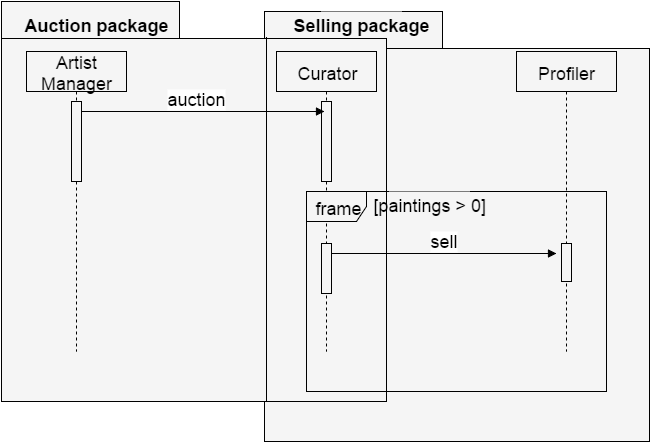
\includegraphics[height=8cm]{media/package.png}
    \caption{Detailed package of model}
    \label{figure:package}
   \end{figure}

   \begin{figure}[ht!]
    \centering
    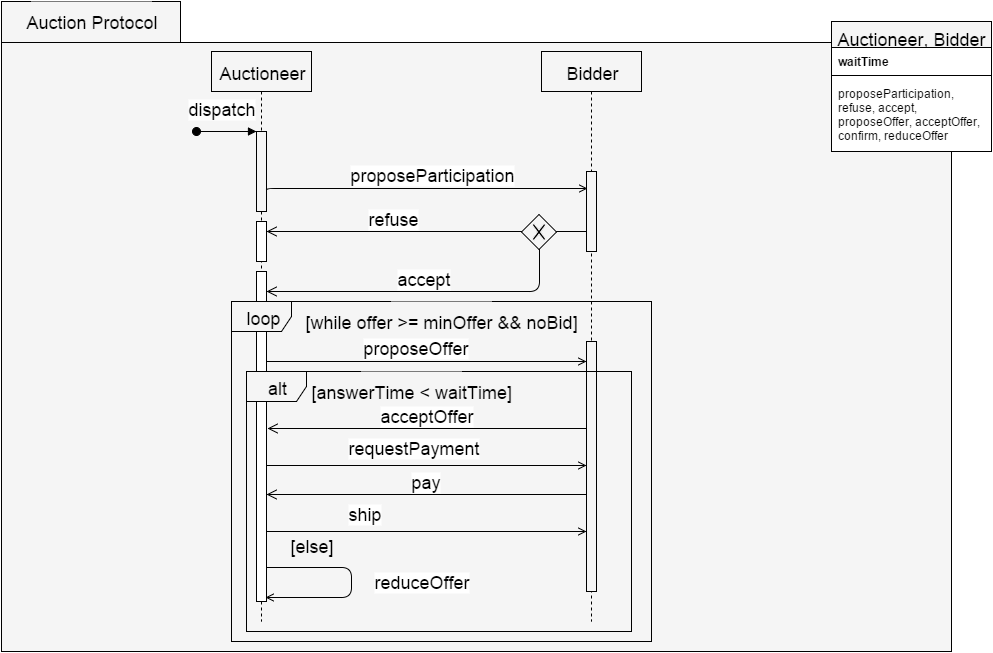
\includegraphics[width=\textwidth]{media/auction_protocol.png}
    \caption{Template for auction protocol}
    \label{figure:auctionProtocol}
   \end{figure}
   
   \begin{figure}[ht!]
    \centering
    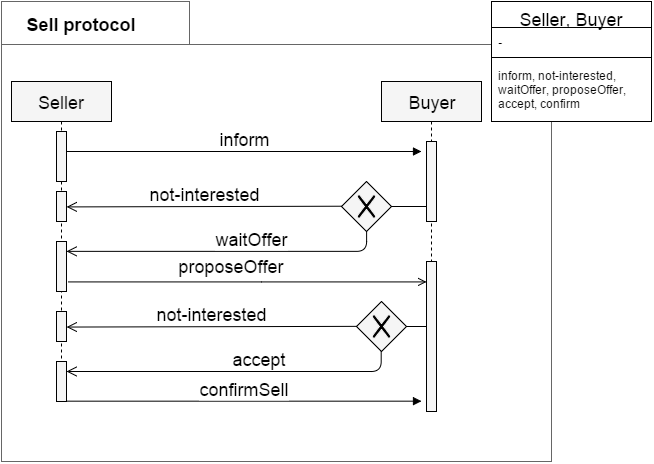
\includegraphics[height=8cm]{media/sell_protocol.png}
    \caption{Template for sell protocol}
    \label{figure:sellProtocol}
   \end{figure}
  
  \subsection{Interactions among agents}
  Three types of agents are present in our model: \textit{Artist Manager}, \textit{Curator}
  and \textit{Profiler}. Figure~\ref{figure:extSeqDiag} displays the interactions between
  the agents. We observe that Curator is the only agent who has two roles in two
  different protocols. The role change takes place once the auction is finished and
  the the Curator has something to sell. Moreover, another important aspect are the concurrent
  messages sent from the Artist Manager to the 2 Curators. They reflect the ``calls`` done
  in an auction.
  
     \begin{figure}[ht!]
    \centering
    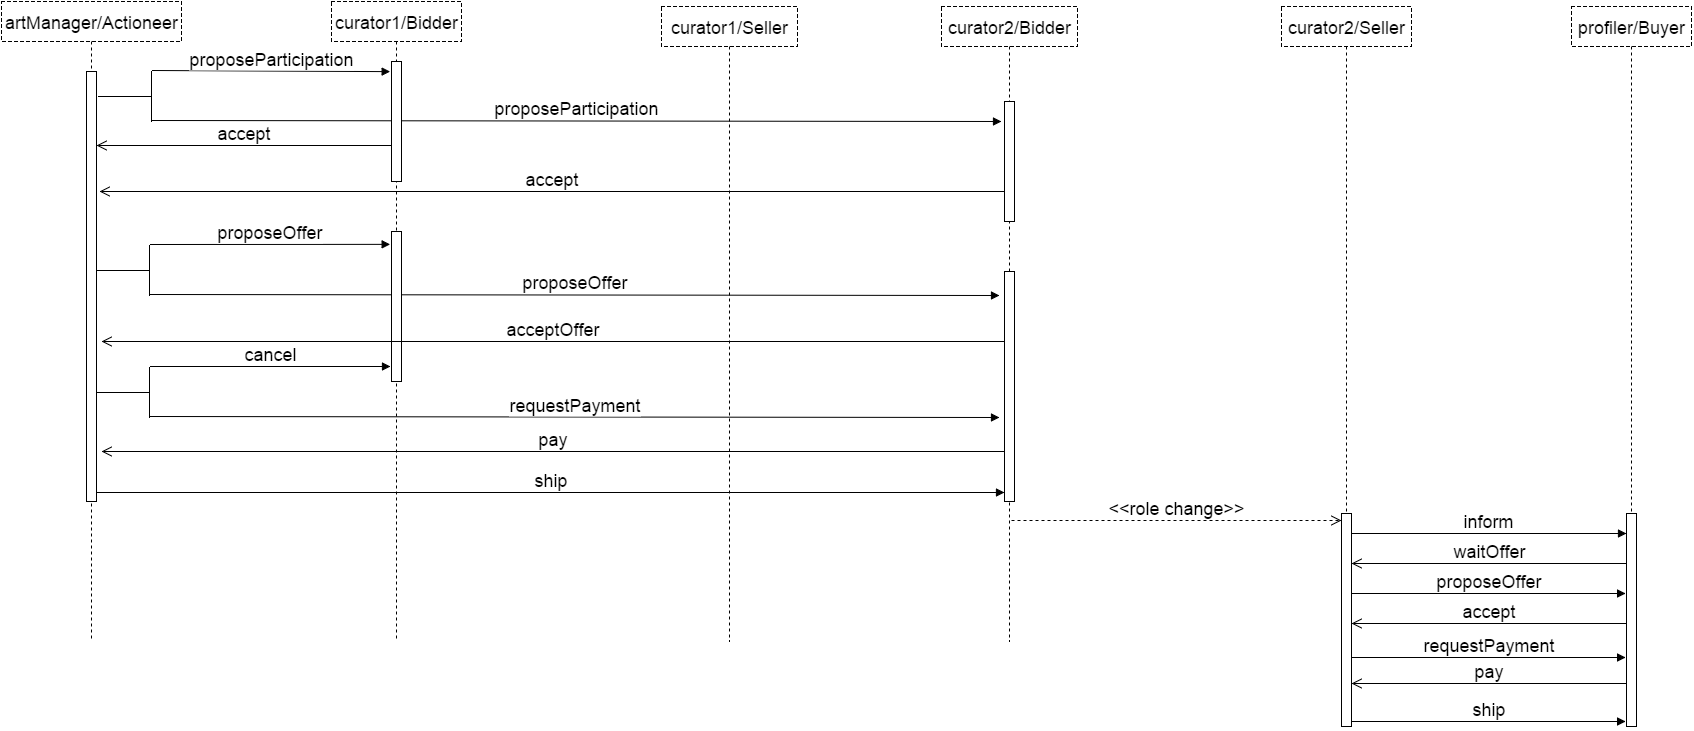
\includegraphics[width=\textwidth]{media/extended_seq_diag.png}
    \caption{Extended sequence diagram}
    \label{figure:extSeqDiag}
   \end{figure}
  
  \subsection{Internal agent processing}
  The internal agent processing is shown by statecharts. One diagram was created for every
  agent type. It is worth mentioning that a \textit{Canceled} state exists in every
  statechart. Moreover, as previously stated the Curator has two distinctive roles
  and this can observed in his statechart as well.
  
   \begin{figure}[ht!]
    \centering
    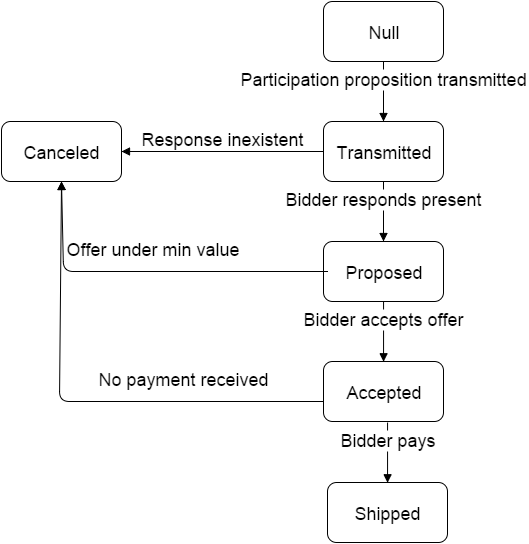
\includegraphics[height=8cm]{media/statechart_artistM.png}
    \caption{Internal process of Artist Manager}
    \label{figure:statechartArtistM}
   \end{figure}
   
   \begin{figure}[ht!]
    \centering
    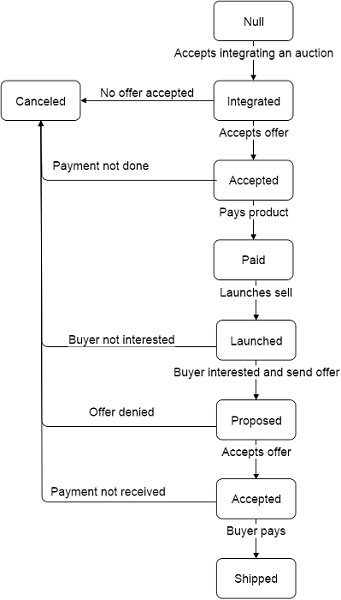
\includegraphics[height=0.9\textheight]{media/statechart_curator.png}
    \caption{Internal process of Curator}
    \label{figure:statechartCurator}
   \end{figure}

   \begin{figure}[ht!]
    \centering
    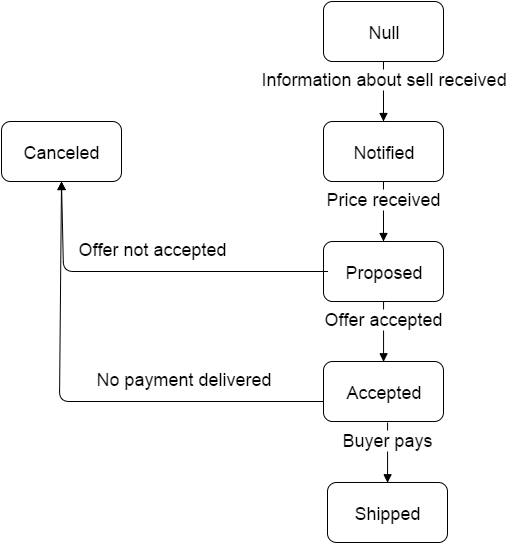
\includegraphics[width=0.9\textwidth]{media/statechart_profiler.png}
    \caption{Internal process of Profiler}
    \label{figure:statechartProfiler}
   \end{figure}
   
  %%%%%%
  
  
  \section{Behaviors design} % task 3
  The behaviors of agents can be designed through UML class diagrams. Figures 
  ~\ref{figure:classArtistManager}, ~\ref{figure:classCurator} and ~\ref{figure:classProfiler}
  show the diagrams for the 3 types of agents found in our model. Such a behavior
  is described by the following elements. Firstly, we have a state description which 
  outlines the specific elements of the agent as well as those which are persistent. Next, 
  are the actions which can be launched by messages (<<re-active>>) or generated by an inner change
  in the agent (<<pro-active>>). The methods are used to do basic changes in the agent class.
  The communication between agents is realized using protocols which are also listed in this UML class. They
  are accompanied by the associated ontology. Consequently, the communication acts (CAs) are listed
  together with their protocol.
  \paragraph{Artist Manager Agent} This agent present in Figure ~\ref{figure:classArtistManager} 
  identifies himself only with one role: Auctioneer. 
  As a particularity, we notice as a persistent field the painting that he possses
  and the permanent goal of the agent. The latter can be translated as selling at a higher price a low
  quality product. This can be seen as a general rule in a selling action. 
  Consequently, the actual goal can be adapted by using the associated method
  according to the permanent one and to a current strategy of the agent.
  \paragraph{Curator Agent} This agent might be considered the most complex one and his behavior
  is represented in Figure ~\ref{classCurator}. The complexity is due to a double role played in the
  given model: Bidder and Seller. Consequently, his state contains strategies for both roles played
  which can be defined through methods. It also contains a persistent field for the budget which can
  be used to purchase a painting. As the curator can change the price after winning an auction, a
  method was introduced which is in charge of this.
  \paragraph{Profiler Agent} The Buyer role is associated to this agent. Behavior is outlined in
  Figure ~\ref{figure:classProfiler}. A budget is also persistent in order to participate in the
  selling protocol. The profiler also has a strategy which can be adapted and the particularity of this
  agent is the presence of a \textit{revealQuality} method. It is used after a purchase in order
  to identify the quality of a painting.
  
   \begin{figure}[ht!]
    \centering
    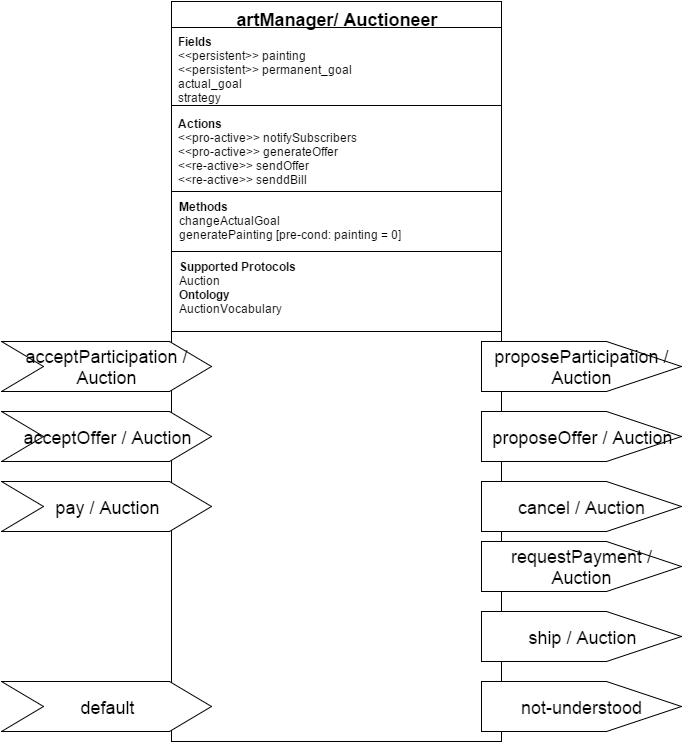
\includegraphics[width=0.9\textwidth]{media/artistManager_class.png}
    \caption{UML class for Artist Manager}
    \label{figure:classArtistManager}
   \end{figure}
   
   \begin{figure}[ht!]
    \centering
    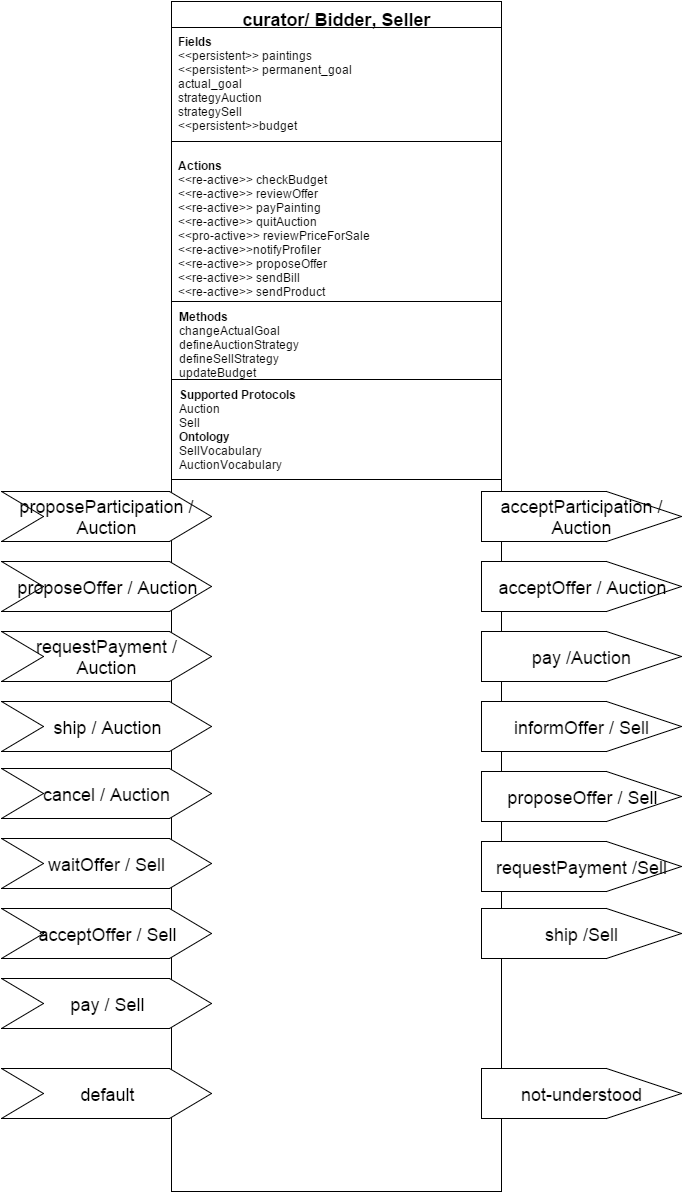
\includegraphics[width=0.9\textwidth]{media/curator_class.png}
    \caption{UML class for Curator}
    \label{figure:classCurator}
   \end{figure}
   
   \begin{figure}[ht!]
    \centering
    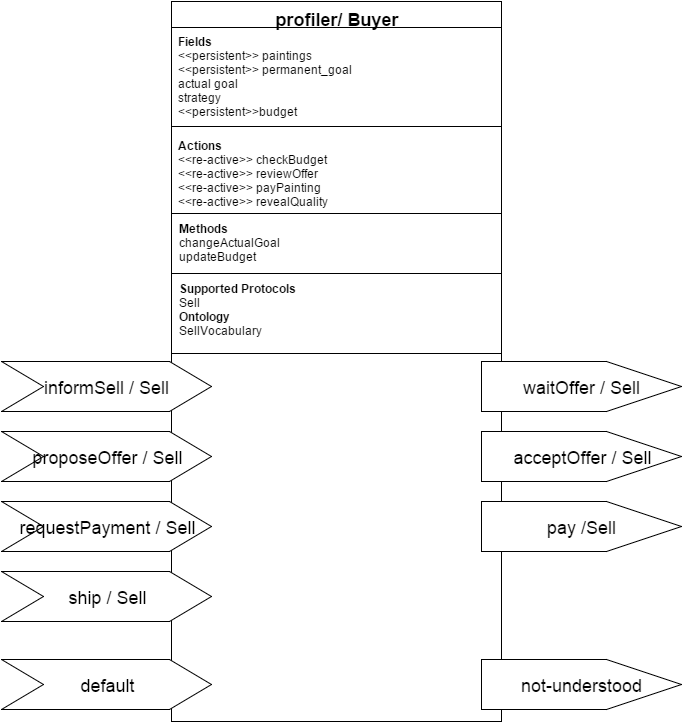
\includegraphics[width=0.9\textwidth]{media/profiler_class.png}
    \caption{UML class for Profiler}
    \label{figure:classProfiler}
   \end{figure}
  
  %%%%%%
  
  \section{Role-based modeling} % task 4
  % Model your system using "Role based modeling" approach
  
  \subsection{RoMAS}
  % TODO Task 4.1 Perform role-based modeling using
  %               RoMAS for the initial task.
  
  \subsubsection{Use cases}
  % (1) Captures use cases;
   
  % Actors:
  % - Product chooser
  % - Auctioneer (DutchAuction)
  % - Bidder (DutchAuction)
  % - Strategist
  % - Proposer
  % - Decision Maker
  % - Buyer
  % - Rejecter
  % - Revealer
  % - Mover
  
  % Use cases:
  % - Choose product (high or low quality)
  % - Auctioneer (DutchAuction): Call for proposal / Manage proposals / Accept proposal / Refuse proposal(s)
  % - Bidder (DutchAuction): Propose
  % - Choose strategy
  % - Define a new price
  % - Propose an offer (product + price)
  % - Decision maker => Define budget
  % - Buy a product
  % - Reject a product
  % - Reveal quality (Buy a product)
  % - Move to Office
  % - Move to House
  % - Move to Museum
  
  In order to realize use cases diagrams, it was to necessary to find out each actor 
  of the scenario. The granularity of actors has been reduced compared to GAIA analysis 
  due to ``atomicness'' of RoMAS method. Use cases are described in Figure~\ref{figure:use_cases}.
  
  \begin{figure}[ht!]
    \begin{subfigure}{0.5\textwidth}
       \centering
       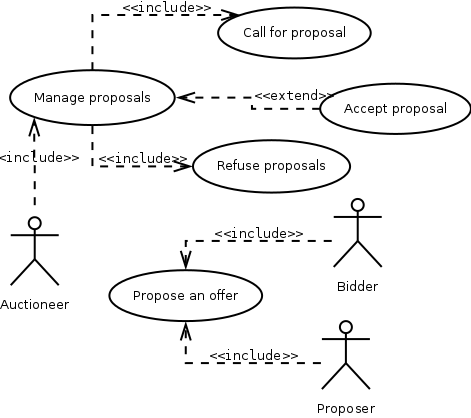
\includegraphics[width=\textwidth]{media/use_cases_1.png}
       \caption{Auctioneer, Bidder and Proposer use cases}
       \label{figure:use_cases_1}
    \end{subfigure}
    \begin{subfigure}{0.5\textwidth}
       \centering
       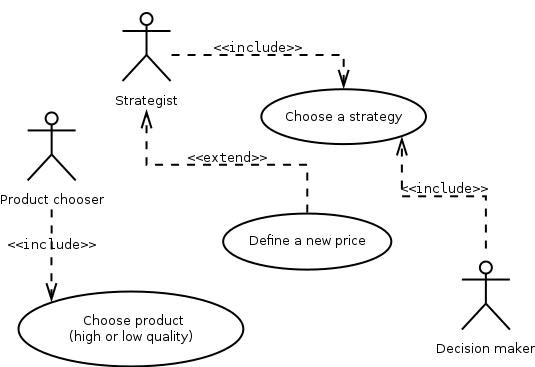
\includegraphics[width=\textwidth]{media/use_cases_2.png}
       \caption{Product choose, Strategist and Decision maker use cases}
       \label{figure:use_cases_2}
    \end{subfigure}
    
    \begin{subfigure}{0.5\textwidth}
       \centering
       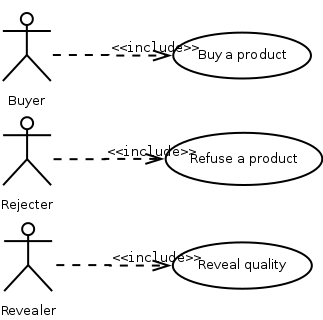
\includegraphics[width=\textwidth]{media/use_cases_3.png}
       \caption{Buyer, Rejecter, Revealer use cases}
       \label{figure:use_cases_3}
    \end{subfigure}
    \begin{subfigure}{0.5\textwidth}
       \centering
       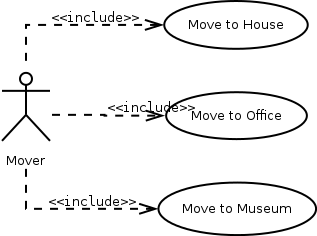
\includegraphics[width=\textwidth]{media/use_cases_4.png}
       \caption{Mover use cases}
       \label{figure:use_cases_4}
    \end{subfigure}

    \caption{Use cases}
    \label{figure:use_cases}
  \end{figure}

  
  \subsubsection{Roles}
  % (2) Identify roles from use cases;
  % Goals / Attributes / Services (methods)
  
  Use cases allow us to identify each role. Each role has a goal, a set of attributes 
  and a set of services. Following paragraphs describe all of them.
  
  % Roles:
  % - Product chooser : product list / getHighQuality / getLowQuality
  % - Auctioneer (DutchAuction) : call for proposal (price) / accept / refuse
  % - Bidder (DutchAuction) : propose / bid
  % - Strategist : strategy list / choose strategy / define new price
  % - Proposer : propose offer
  % - Decision maker: budget / define budget / choose action(proposal)
  % - Buyer : buy product
  % - Rejecter : reject product
  % - Revealer : reveal quality
  % - Mover : move to house / move to office / move to museum
  
  \begin{multicols}{2}
  %%%
  \begin{mdframed}
  \textbf{Product chooser}'s main goal is to select a product within a list of different 
  products. It is possible to select a high or a low quality product in order to sell it 
  later.\\
  Attributes: $<$List$>$Product\\
  Services:\vspace{-5pt}
  \begin{itemize}
    \itemsep0pt
    \item PickHighQualityProduct()
    \item PickLowQualityProduct()
  \end{itemize}
  \end{mdframed}
  %%%
  \begin{mdframed}
  \textbf{Auctioneer}'s main goal is to sell product (high or low quality) using Dutch Auction 
  protocol.\\
  Attributes: Price\\
  Services:\vspace{-5pt}
  \begin{itemize}
    \itemsep0pt
    \item callForProposal(price)
    \item receiveProposal()
    \item acceptProposal()
    \item refuseProposal()
  \end{itemize}
  \end{mdframed}
  %%%
  \begin{mdframed}
  \textbf{Buyer}'s main goal is to buy a product from a \textbf{Proposer}.\\
  Attributes: -\\
  Services: buyProduct()
  \end{mdframed}
  %%%
  \begin{mdframed}
  \textbf{Bidder} (or \textbf{Proposer})'s main goal is to buy product from auctioneer. Product 
  can be high or low quality but this role doesn't have any idea about the quality of the 
  product. Thus, parameters available are: product and price offered. Bidder is specialized 
  in Dutch Auction protocol.\\
  Attributes: -\\
  Services: \vspace{-5pt}
  \begin{itemize}
   \itemsep0pt
   \item propose()
   \item proposePrice(price)
  \end{itemize}
  \end{mdframed}
  %%%
  \begin{mdframed}
  \textbf{Strategist}'s main goal is to provide strategy to define new price and set up affordable 
  prices for buyers and bidders.\\
  Attributes: $<$List$>$ Strategy\\
  Services:\vspace{-5pt}
  \begin{itemize}
    \itemsep0pt
    \item chooseStrategy()
    \item defineNewPrice()
  \end{itemize}
  \end{mdframed}
  %%%
  \begin{mdframed}
  \textbf{Decision maker}'s main goal is to define and manage a budget. Then this 
  role has the opportunity to choose actions to perform next according to strategy 
  defined by \textbf{Strategist}.\\
  Attributes: Budget\\
  Services:\vspace{-5pt}
  \begin{itemize}
    \itemsep0pt
    \item defineBudget()
    \item chooseAction(proposal)
  \end{itemize}
  \end{mdframed}
  %%%
  \begin{mdframed}
  \textbf{Rejecter}'s main goal is to refuse product offered by a \textbf{Proposer}.\\
  Attributes: -\\
  Services: refuseProduct()
  \end{mdframed}
  %%%
  \begin{mdframed}
  \textbf{Revealer}'s main goal is to reveal quality of a product once it has been bought.\\
  Attributes: -\\
  Services: revealQuality()
  \end{mdframed}
  %%%
  \begin{mdframed}
  \textbf{Mover}'s main goal is to move from place to place in order to perform actions.\\
  Attributes: -\\
  Services:\vspace{-10pt}
  \begin{itemize}
    \itemsep0pt
    \item moveToHouse()
    \item moveToOffice()
    \item moveToMuseum()
  \end{itemize}
  \end{mdframed}
  
  \end{multicols}
  
  \subsubsection{Role organization}
  % (3) Constructs role organization;
  % Artist Manager  <-> Curator <-> Profiler
  
  It is possible to aggregate and gather some roles (previously defined) together. Among all 
  of them, 3 main roles appear: \textbf{Artist Manager}, \textbf{Curator} and \textbf{Profiler}. 
  Figure~\ref{figure:role_organization} displays roles organization in smart museum scenario.
  
  \begin{figure}[ht!]
    \centering
    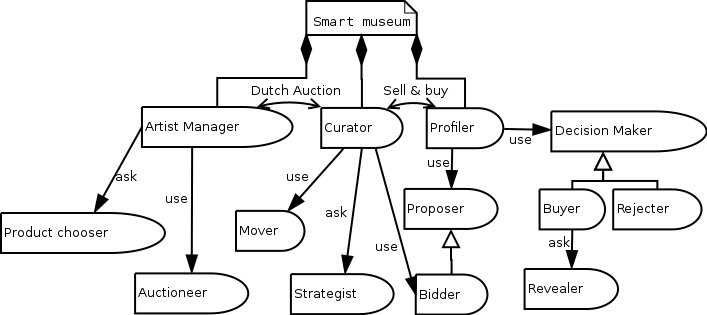
\includegraphics[width=\textwidth]{media/roles_organization.png}
    \caption{Role organization}
    \label{figure:role_organization}
  \end{figure}
  
  
  \subsubsection{Binding roles-agents}
  % (4) For each role, if the appropriate agent 
  %     does not exist, then go to (5); else
  %     I. Binds roles to agents
  %     II. Describes dynamic properties of bind 
  %         relation between agents and roles
  %     III. Go to (6)
  % (5) Generates agents according to roles; Go to (4).I.
  % (6) Generates codes for agents with roles bound;

  For each role, it is possible to bind an appropriate agent. Thanks to the previous part, 
  it is easy to find our agents:
  
  \newcommand{\ama}{\textit{ArtistManagerAgent}}
  \newcommand{\cua}{\textit{CuratorAgent}}
  \newcommand{\proa}{\textit{ProfilerAgent}}
  
  \begin{itemize}
   \itemsep0pt
   \item \ama{}: responsible to choose a product and give it to the \cua{} for the product to 
   be sold. Roles transition are displayed in state diagram in Figure~\ref{figure:role_transition_ama}.
   \item \cua{}: responsible to move from museum to office and then to house in order to 
   act as bidders with \ama{} and then retail product to \proa{}. Roles transition are displayed in 
   state diagram in Figure~\ref{figure:role_transition_cua}.
   \item \proa{}: try to buy products offered by \cua{} at the best prices and reveal its qualities. 
   Roles transition are displayed in state diagram in Figure~\ref{figure:role_transition_proa}.
  \end{itemize}
  

  % Agents TODO define attributes / methods like in Fig. 5 :
  % - ArtistManagerAgent (Product chooser, Auctionner)
  % - CuratorAgent (Bidder, Strategist, Proposer, Mover)
  % - Profiler (Decision maker, Buyer, Rejecter, Revealer)
  
  % Role transition ? => State diagrams
  % - ArtistManagerAgent: Product choose <-> Auctionner
  % - CuratorAgent: Strategist -> Mover -> Bidder -> Mover
  %                 -> Proposer /^/
  % - ProfilerAgent: Decision maker -> Buyer -> Revealer -> Decision maker
  %                                 -> Rejecter -> Decision maker
  \begin{figure}[ht!]
    \centering
    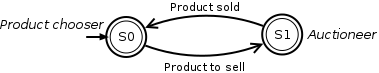
\includegraphics[width=\textwidth]{media/role_transition_ama.png}
    \caption{Roles transition of ArtistManagerAgent}
    \label{figure:role_transition_ama}
  \end{figure}
  
  \begin{figure}[ht!]
    \centering
    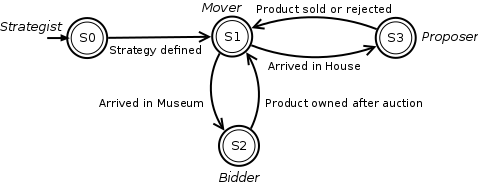
\includegraphics[width=\textwidth]{media/role_transition_cua.png}
    \caption{Roles transition of CuratorAgent}
    \label{figure:role_transition_cua}
  \end{figure}
  
  \begin{figure}[ht!]
    \centering
    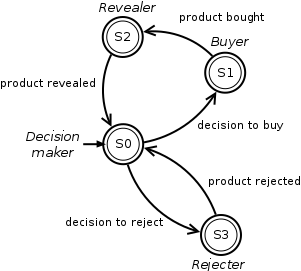
\includegraphics[height=7cm]{media/role_transition_proa.png}
    \caption{Roles transition of ProfilerAgent}
    \label{figure:role_transition_proa}
  \end{figure}

  \subsection{Comparison with GAIA}
  % Task 4.2 Comment on differences in resulting
  %          designs of 4.1 and GAIA (from Task 1).
  % (i.e. Analysis phase of GAIA against performing 
  %  role-based modeling as first step to GAIA analysis)

  Compared to GAIA analysis, role-based modeling (RoMAS) allows dynamic roles 
  for each agent. Based on use cases and actors, it is possible to find out 
  roles in the system. GAIA, on the other hand doesn't provide such method and 
  it goes first in roles definition with 4 different characteristics: responsibilities, 
  permissions, protocols and activities. RoMAS also produces organizational 
  diagram in order to outline roles interactions while GAIA asks for an acquaintance 
  model. Roles are seen as states where it is possible to perform actions (like 
  behaviors in JADE framework) in role-based modeling. As a result, roles are more 
  atomic in RoMAS method than with GAIA analysis which goes deeper in the details with 
  concepts such as protocols and activities. These concepts are very close (if not 
  similar) to the behavior concept.
  
  It is also important to notice that RoMAS doesn't have any method to deal with mobility 
  and it has to be considered as a role. Notions like places and relationships between 
  agents and places don't exist neither.
  
  % TODO well ? :p
  Finally, RoMAS is at MAS analysis methods what Ruby is at Object Oriented Programing 
  languages: ``Everything is role''
  %%%%%%
  
  
  \section{JADE and other agent platforms} % task 5
  % There are number of implementations of agent platforms which conform to 
  % FIPA specifications. Perform a comparison of at least 2 other agent 
  % platforms with JADE
  
  % Some other platforms: Agent Development Kit, FIPA-OS, 
  %                       Jack Intelligent Agents, ZEUS, 
  %                       SAGE, ...
  % TODO choose 2 of them
  
  % Links:
  % - https://en.wikipedia.org/wiki/FIPA
  
  
  There are several multi-agents platform respecting and implementing FIPA 
  specifications. Among all of them, we choose to study \textbf{Jack Intelligent 
  Agents} and \textbf{TODO}. % TODO
  
  \subsection{Jack Intelligent Agents}
  % refs:
  % - https://en.wikipedia.org/wiki/JACK_Intelligent_Agents
  % - http://www.aosgrp.com/documentation/jack/Agent_Manual_WEB/index.html#Introduction
  
  \subsubsection{Architecture}
  % TODO Architecture of platform
  
  \subsubsection{Services provided}
  % TODO Services provided by platform
  
  \subsubsection{Simple scenario}
  % TODO Comparison of implementation of a simple scenario same as Question 2 (??)
  % (i.e. service implementation, service registration and service discovery)
  
  \subsubsection{Notable projects}
  % TODO List some notable projects which use that platform
  
  \subsubsection{Personnel opinion}
  % TODO Your personnel opinion/judgment about the platform as compared to JADE
  % Yo can take part 3 (simple scenario) as your starting point, and explain the 
  % architecture and services the platform provides from a practical point of view
  
  \clearpage % TODO to remove
  
  \subsection{platform 2} % TODO to choose 
  
  \subsubsection{Architecture}
  % TODO Architecture of platform
  
  \subsubsection{Services provided}
  % TODO Services provided by platform
  
  \subsubsection{Simple scenario}
  % TODO Comparison of implementation of a simple scenario same as Question 2 (??)
  % (i.e. service implementation, service registration and service discovery)
  
  \subsubsection{Notable projects}
  % TODO List some notable projects which use that platform
  
  \subsubsection{Personnel opinion}
  % TODO Your personnel opinion/judgment about the platform as compared to JADE
  % Yo can take part 3 (simple scenario) as your starting point, and explain the 
  % architecture and services the platform provides from a practical point of view
  
  
  %%%%%%
  
  
  \section{Conclusion}
  % TODO what this project gave us ?
  In this project, we discovered several methods to model multi-agents system. We also 
  introduced 2 MAS platforms and compared both of them with JADE framework.

  
% bibliography
%\bibliographystyle{plainurl}
%\bibliography{references}

\end{document}